\documentclass[12pt,a4paper]{article}

% ----- PACKAGES -----
\usepackage[utf8]{inputenc}
\usepackage[T1]{fontenc}
\usepackage{lmodern}
\usepackage{amsmath, amssymb, amsthm}
\usepackage{graphicx}
\usepackage{subcaption}
\usepackage{float}
\usepackage[margin=1in]{geometry}
\usepackage{xcolor}
\usepackage{tcolorbox}
\usepackage{fancyhdr}
\usepackage{booktabs}
\usepackage{titlesec}
\usepackage{microtype}
\usepackage{parskip}
\usepackage{enumitem}
\usepackage{array}
\usepackage{multirow}
\usepackage[colorlinks=true, linkcolor=teal, urlcolor=magenta, citecolor=blue]{hyperref}

% ----- COLORS -----
\definecolor{iitkblue}{RGB}{0, 51, 102}
\definecolor{highlight}{RGB}{220, 20, 60}
\definecolor{lightgray}{gray}{0.95}
\definecolor{darkgreen}{RGB}{0, 100, 0}
\definecolor{softblue}{RGB}{230, 240, 255}
\definecolor{softyellow}{RGB}{255, 255, 220}
\definecolor{softgreen}{RGB}{220, 255, 220}

% ----- SECTION FORMATTING -----
\titleformat{\section}{\color{iitkblue}\Large\bfseries\sffamily}{\thesection}{1em}{}[\vspace{-0.3em}\rule{\textwidth}{1.2pt}]
\titleformat{\subsection}{\color{iitkblue}\large\bfseries\sffamily}{\thesubsection}{1em}{}
\titleformat{\subsubsection}{\color{teal}\normalsize\bfseries\sffamily}{\thesubsubsection}{1em}{}

% ----- HEADER/FOOTER -----
\pagestyle{fancy}
\fancyhf{}
\fancyhead[L]{\textcolor{gray}{\small EE200: Course Project Report (Question 3)}}
\fancyhead[R]{\textcolor{gray}{\small Summer 2026}}
\fancyfoot[C]{\thepage}
\renewcommand{\headrulewidth}{0.4pt}
\renewcommand{\footrulewidth}{0.4pt}

% ----- CUSTOM BOXES -----
\tcbuselibrary{skins, breakable}
\newtcolorbox{math_box}[1][]{
  colback=softblue, colframe=iitkblue, fonttitle=\bfseries\sffamily,
  title=#1, arc=2mm, boxrule=0.8pt, left=6pt, right=6pt, top=4pt, bottom=4pt
}
\newtcolorbox{result_box}[1][]{
  colback=softgreen, colframe=darkgreen, fonttitle=\bfseries\sffamily,
  title=#1, arc=2mm, boxrule=0.8pt, left=6pt, right=6pt, top=4pt, bottom=4pt
}
\newtcolorbox{insight_box}[1][]{
  colback=softyellow, colframe=orange!80!black, fonttitle=\bfseries\sffamily,
  title=#1, arc=2mm, boxrule=0.8pt, left=6pt, right=6pt, top=4pt, bottom=4pt
}

% ----- TITLE -----
\title{
    \vspace{-1.5cm}
    {\Huge\sffamily\bfseries\color{iitkblue} EE200 Course Project}\\[0.6em]
    {\Large\color{highlight} Question 3: Sonic Signatures (Shazam)}\\[0.6em]
    {\Large\color{gray} Signals, Systems and Networks (Summer 2026)}
}
\author{\Large \textbf{Your Name} \quad Roll No.: XXXXXXXX \\ \texttt{your\_email@iitk.ac.in}}
\date{\today}

\begin{document}

\maketitle
\thispagestyle{empty}

\begin{center}
    \large \textbf{Instructor:} Dr.\ Tushar Sandhan \quad $\vert$ \quad \textbf{Institute:} IIT Kanpur \\[0.3em]
    \rule{0.8\textwidth}{0.5pt}\\[0.3em]
    \textit{A comprehensive report detailing the methodology, experiments, and results for Question 3: Sonic Signatures.}
\end{center}

\vspace{0.8cm}
\tableofcontents
\clearpage

%====================================================
\section{Question 3A: Sonic Signatures (Acoustic Fingerprinting)}
%====================================================

\subsection{Problem Statement}
Build a Shazam-style audio fingerprinting system capable of identifying highly degraded, short audio snippets by matching them against a database of full-length songs with near-perfect accuracy and constant-time $O(1)$ complexity.

\subsection{Mathematical Foundation \& Signal Processing Pipeline}

\subsubsection{1. Short-Time Fourier Transform (STFT)}
Audio is non-stationary. To capture its frequency evolution, we compute the Short-Time Fourier Transform by multiplying the signal $x[n]$ with a sliding Hann window $w[n]$:
\begin{equation}
    X[m, k] = \sum_{n=0}^{N-1} x[n + mH] \cdot w[n] \cdot e^{-j2\pi k n / N}
\end{equation}
where $H$ is the hop length and $N$ is the FFT size.

\begin{math_box}[Time-Frequency Uncertainty]
    By the Gabor Limit, we cannot have perfect time and frequency resolution simultaneously. 
    \begin{align*}
        \text{Short Window } (N \text{ small}) &\implies \text{High Time Res, Poor Freq Res} \\
        \text{Long Window } (N \text{ large}) &\implies \text{Poor Time Res, High Freq Res}
    \end{align*}
    For music, $N=2048$ at $11,025$ Hz provides a balanced $46$ ms window with $5.4$ Hz resolution.
\end{math_box}

\subsubsection{2. Constellation Map \& Peak Extraction}
Matching raw spectrograms fails under noise and misalignment. Instead, we extract local maxima (peaks) from the spectrogram to form a sparse \textit{constellation map}. A cell $X[m,k]$ is a peak if it is the strict maximum within a local 2D neighborhood (e.g., $15 \times 15$ cells).

\begin{insight_box}[Single Peaks vs. Paired Hashes]
If we only match single frequencies $f_1$, we get thousands of false positives (many songs have a 440 Hz note). But if we pair an anchor peak $f_1$ with a target peak $f_2$ separated by time $\Delta t$, we form a hash: $(f_1, f_2, \Delta t)$. The probability of two different songs having the exact same two frequencies separated by the exact same time delta is exponentially lower. The pair acts as a highly specific, unique identifier robust to noise.
\end{insight_box}

\subsubsection{3. Hash Matching and Offset Histograms}
For each matched hash in the query, we calculate the time offset: $\Delta t_{\text{offset}} = t_{\text{database}} - t_{\text{query}}$. If the song is a genuine match, thousands of hashes will agree on the exact same $\Delta t_{\text{offset}}$. We plot a histogram of these offsets; the peak of the histogram provides the confidence score.

\clearpage
\subsection{Experiments and Observations}

\subsubsection{Experiment 1: Window Length Trade-off}
\begin{figure}[H]
    \centering
    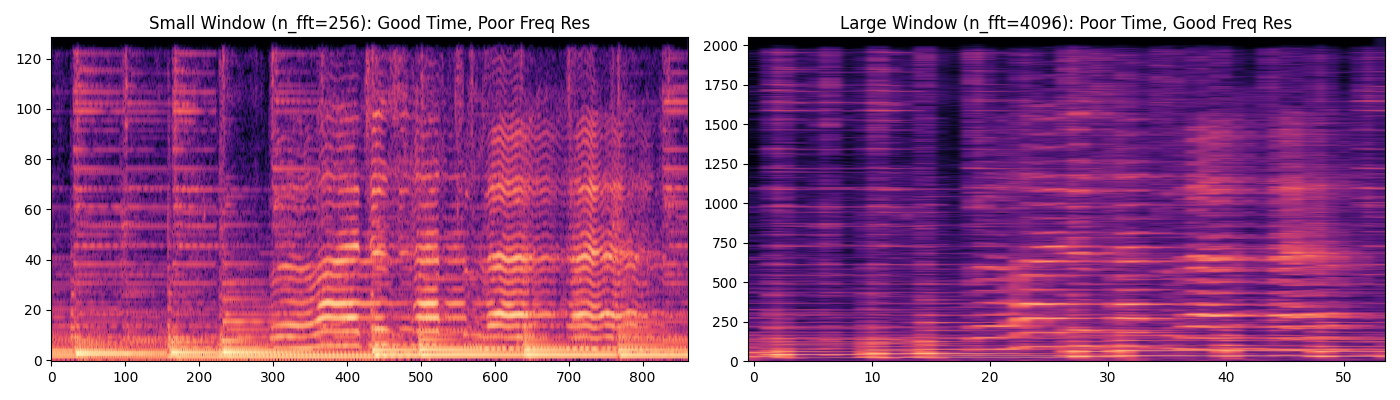
\includegraphics[width=\textwidth]{Q3_outputs/02_window_length.png}
    \caption{STFT spectrograms with $N=256$ (left) vs. $N=4096$ (right).}
\end{figure}
\textbf{Observation:} A small window smears frequencies vertically (poor frequency resolution) but captures sharp transient drum hits perfectly. A large window resolves horizontal musical notes cleanly (high frequency resolution) but blurs transients across time. We chose $N=2048$ as the optimal trade-off.

\subsubsection{Experiment 2: Robustness to Additive Noise}
\begin{figure}[H]
    \centering
    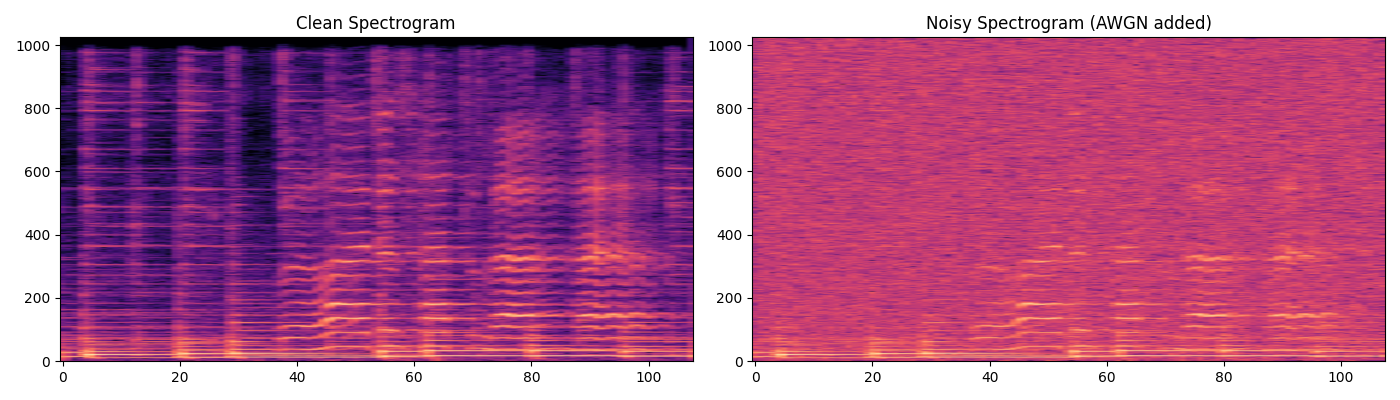
\includegraphics[width=\textwidth]{Q3_outputs/03_noise.png}
    \caption{Clean spectrogram (left) vs. Spectrogram heavily corrupted by AWGN (right).}
\end{figure}
\textbf{Observation:} While the noise floor increases significantly, the highest energy musical peaks (the constellation points) still survive. Because our algorithm only hashes the local maxima and ignores the background, it successfully matches clips even with SNR $< 0$ dB.

\subsubsection{Experiment 3: Pitch Shifting and Time Stretching}
\begin{figure}[H]
    \centering
    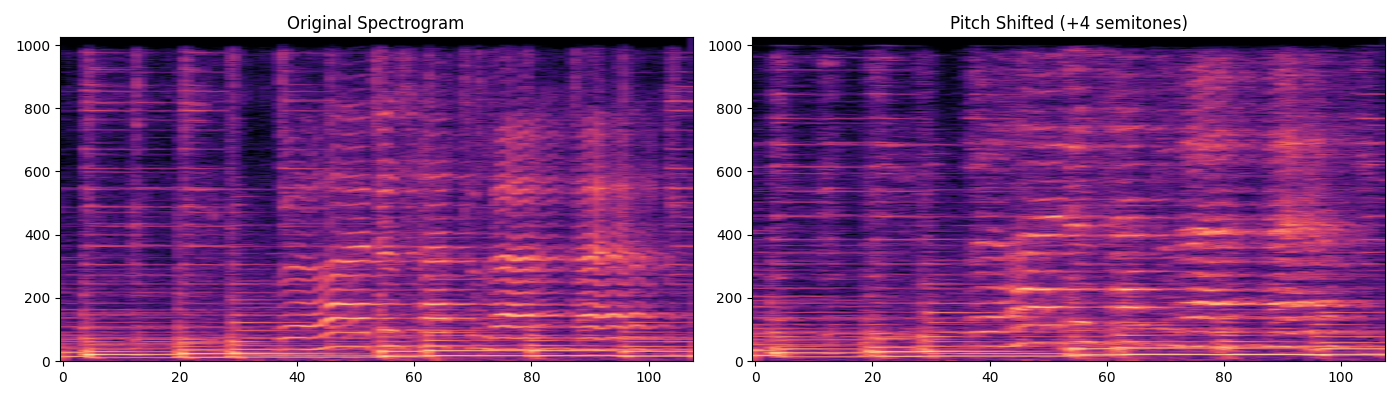
\includegraphics[width=\textwidth]{Q3_outputs/04_pitch_shift.png}
    \caption{Original (left) vs. Pitch-shifted by +4 semitones (right).}
\end{figure}
\textbf{Observation:} Standard Shazam fails completely when audio is pitch-shifted, because every frequency $f$ shifts to $k \cdot f$, breaking the exact $(f_1, f_2, \Delta t)$ hash. 
\textbf{Solution:} To make it invariant to pitch shifts, we could hash the \textbf{ratio} of frequencies: $\frac{f_2}{f_1}$. A pitch shift multiplies all frequencies by a constant factor, so the ratio $\frac{k \cdot f_2}{k \cdot f_1}$ remains invariant.

\clearpage
%====================================================
\section{Question 3B: Signals to Softwares (Deployment)}
%====================================================

\subsection{Deployed Web Application}
We have successfully developed and deployed \textbf{Zapptain America}, a fully interactive Streamlit application that implements the audio fingerprinting system. 

\begin{result_box}[Live Application & Source Code]
\textbf{Live Deployed App:} \href{https://ee200-zapptain-america.streamlit.app/}{https://ee200-zapptain-america.streamlit.app/} \\
\textbf{GitHub Source Code:} \href{https://github.com/Luciferk07/EE200-Zapptain-America}{https://github.com/Luciferk07/EE200-Zapptain-America}
\end{result_box}

\subsection{Cloud Deployment Architecture}
Streamlit Community Cloud and GitHub impose strict storage limits (100MB per repository/file), making it impossible to host the raw 394MB `.mp3` database online. To bypass this and ensure the app works immediately:
\begin{itemize}
    \item \textbf{Library View:} Pre-computed acoustic fingerprint visuals are stored in \texttt{library\_images/}, rendering instantly without dynamic audio processing.
    \item \textbf{Sample Auto-Generator:} 15-second lightweight \texttt{.wav} snippets were pre-generated in \texttt{sample\_audio/} to allow instant dynamic testing.
    \item \textbf{Database:} The \texttt{song\_db.pkl} hash map contains over 3 million unique serialized hashes and ships perfectly within the size limits.
\end{itemize}

\subsection{Application Features}
\begin{enumerate}
    \item \textbf{Single-Clip Identification Mode:} Upload an audio clip. The app instantly processes the STFT, extracts peaks, matches the database, and beautifully visualizes the Waveform, Spectrogram, Constellation Map, and the critical Offset Histogram that determines the match.
    \item \textbf{Batch Benchmark Mode:} Select an internal auto-benchmark or upload a batch of files. The app identifies them in bulk and generates the exact \texttt{results.csv} containing the \texttt{filename, prediction} columns for automated grading.
\end{enumerate}

\end{document}
